%!TEX root = main.tex
\section{The Fuzzy Setting: Towards Intelligent Visual Search}\label{sec:vague}
\agp{We don't really say all that much about the 5 discovery goals
in this section or the next. One option is to de-emphasize it throughout, or at least
get rid of the table.}
\dor{Is it sufficient highlight which discovery goals is covered by the tools that we discuss and how? It might also help to italicize and use a single consistent term for describing each discovery goal: \textit{Compare}, Identifying patterns as \textit{Diagonose}? , Cluster/Outliers as \textit{Overview}?, \textit{Summarize},\textit{Explain}}. 
\par As we argued in the previous section \agp{provide a connection}

\subsection{The Challenge of Usability-Expressiveness Tradeoff}
\par The challenge for supporting vague and 
complex querying stems from the inevitable design trade-off between query expressiveness and interface usability in interactive data exploration systems~\cite{Jagadish2007,Morton2014}. This tradeoff is observed not only in visual data exploration systems, but also true for general ad-hoc data querying. While querying language such as SQL are highly expressive, formulating SQL queries that maps user's high-level intentions to specific query statements is challenging~\cite{Jagadish2007,Khoussainova2010}. As a result, query construction interfaces have been developed to address this issue by enabling direct manipulation of queries through graphical representations~\cite{Abouzied2012}, gestural interaction~\cite{Nandi2013}, and tabular inputs~\cite{Zloof1975,Embley1989}. For example, form-based query builders often consist of highly-usable interfaces that ask users for a specific set of information mapped onto a pre-defined query. However, form-based query builders are often based on query templates with limited expressiveness in their semantic and conceptual coverage, which makes it difficult for expert users to express complex queries. The extensibility of these systems also comes with high engineering costs, as well as potentially overloading users with too many potential options to chose from. Thus, there is a need for tools that enable users to formulate rich and complex queries, yet amenable to the fuzzy, imprecise query inputs that users might naturally formulate. 
%users mhighly usable even for novices.  
%Most systems design exhibits a trade-off between how expressive can the query be and how usable the interface is. 

% \begin{itemize}
% \item Inferring user intent in querying and context is important (both in terms of user input and what is recommended)
% \item tools can not assume user has querying intention. exploration without intention, user don’t know what they are searching for --> Recommendation.
% \item The important thing here is identifying what should be done by the system v.s. requested from user. Inappropriate choice of these will result in lack of expressibility and user feeling lack of control of analysis, limiting exploration.
% \item 
% \end{itemize}
%we can not assume a one-size-fit-all system that could fit the needs for users of different expertise levels and workloads. In this section, 

\agp{One issue with the way this section is written is that the related work discussion is embedded within the research challenges. While this is fine, it deviates from the way the other sections are written. If there is a way we can make this uniform and consistent, that would be valuable.}
\subsection{Ongoing Work and Research Challenges within the Fuzzy Setting}
\par Given the tradeoff between expressiveness and usability, we discuss a growing class of systems that accelerates the discovery process of answering imprecise, fuzzy, and complex queries, with many open research questions including: {\em How can we develop better ways to resolve ambiguity by inferring the information needs and intent of analysts? What is the appropriate level of feedback and interactions for query refinement? How can we develop interpretable visual metaphors that explain how the query was interpreted and why specific query results are returned?} 

We describe three different system challenges in interpreting fuzzy, complex queries. Since these systems operate in the intermediate layer between users and \vidaql as shown in Figure~\ref{fig:vida_architecture}, we use the linguistical classification scheme to provide an analogy for where the ambiguous aspects of queries may arise, noting that the use of this analogy by no means limits our analysis to only natural language interfaces.
\agp{One concern is that we're talking about systems that support visualization specification, or dialog, but none of them talk about visualization search. We should clarify that these systems are only described because they have encountered similar challenges, but our challenges will be broader and harder to optimize.}
%they emit Since most visual query systems operate on top of a querying language, %during visual data exploration

\begin{figure}[h!]
\centering
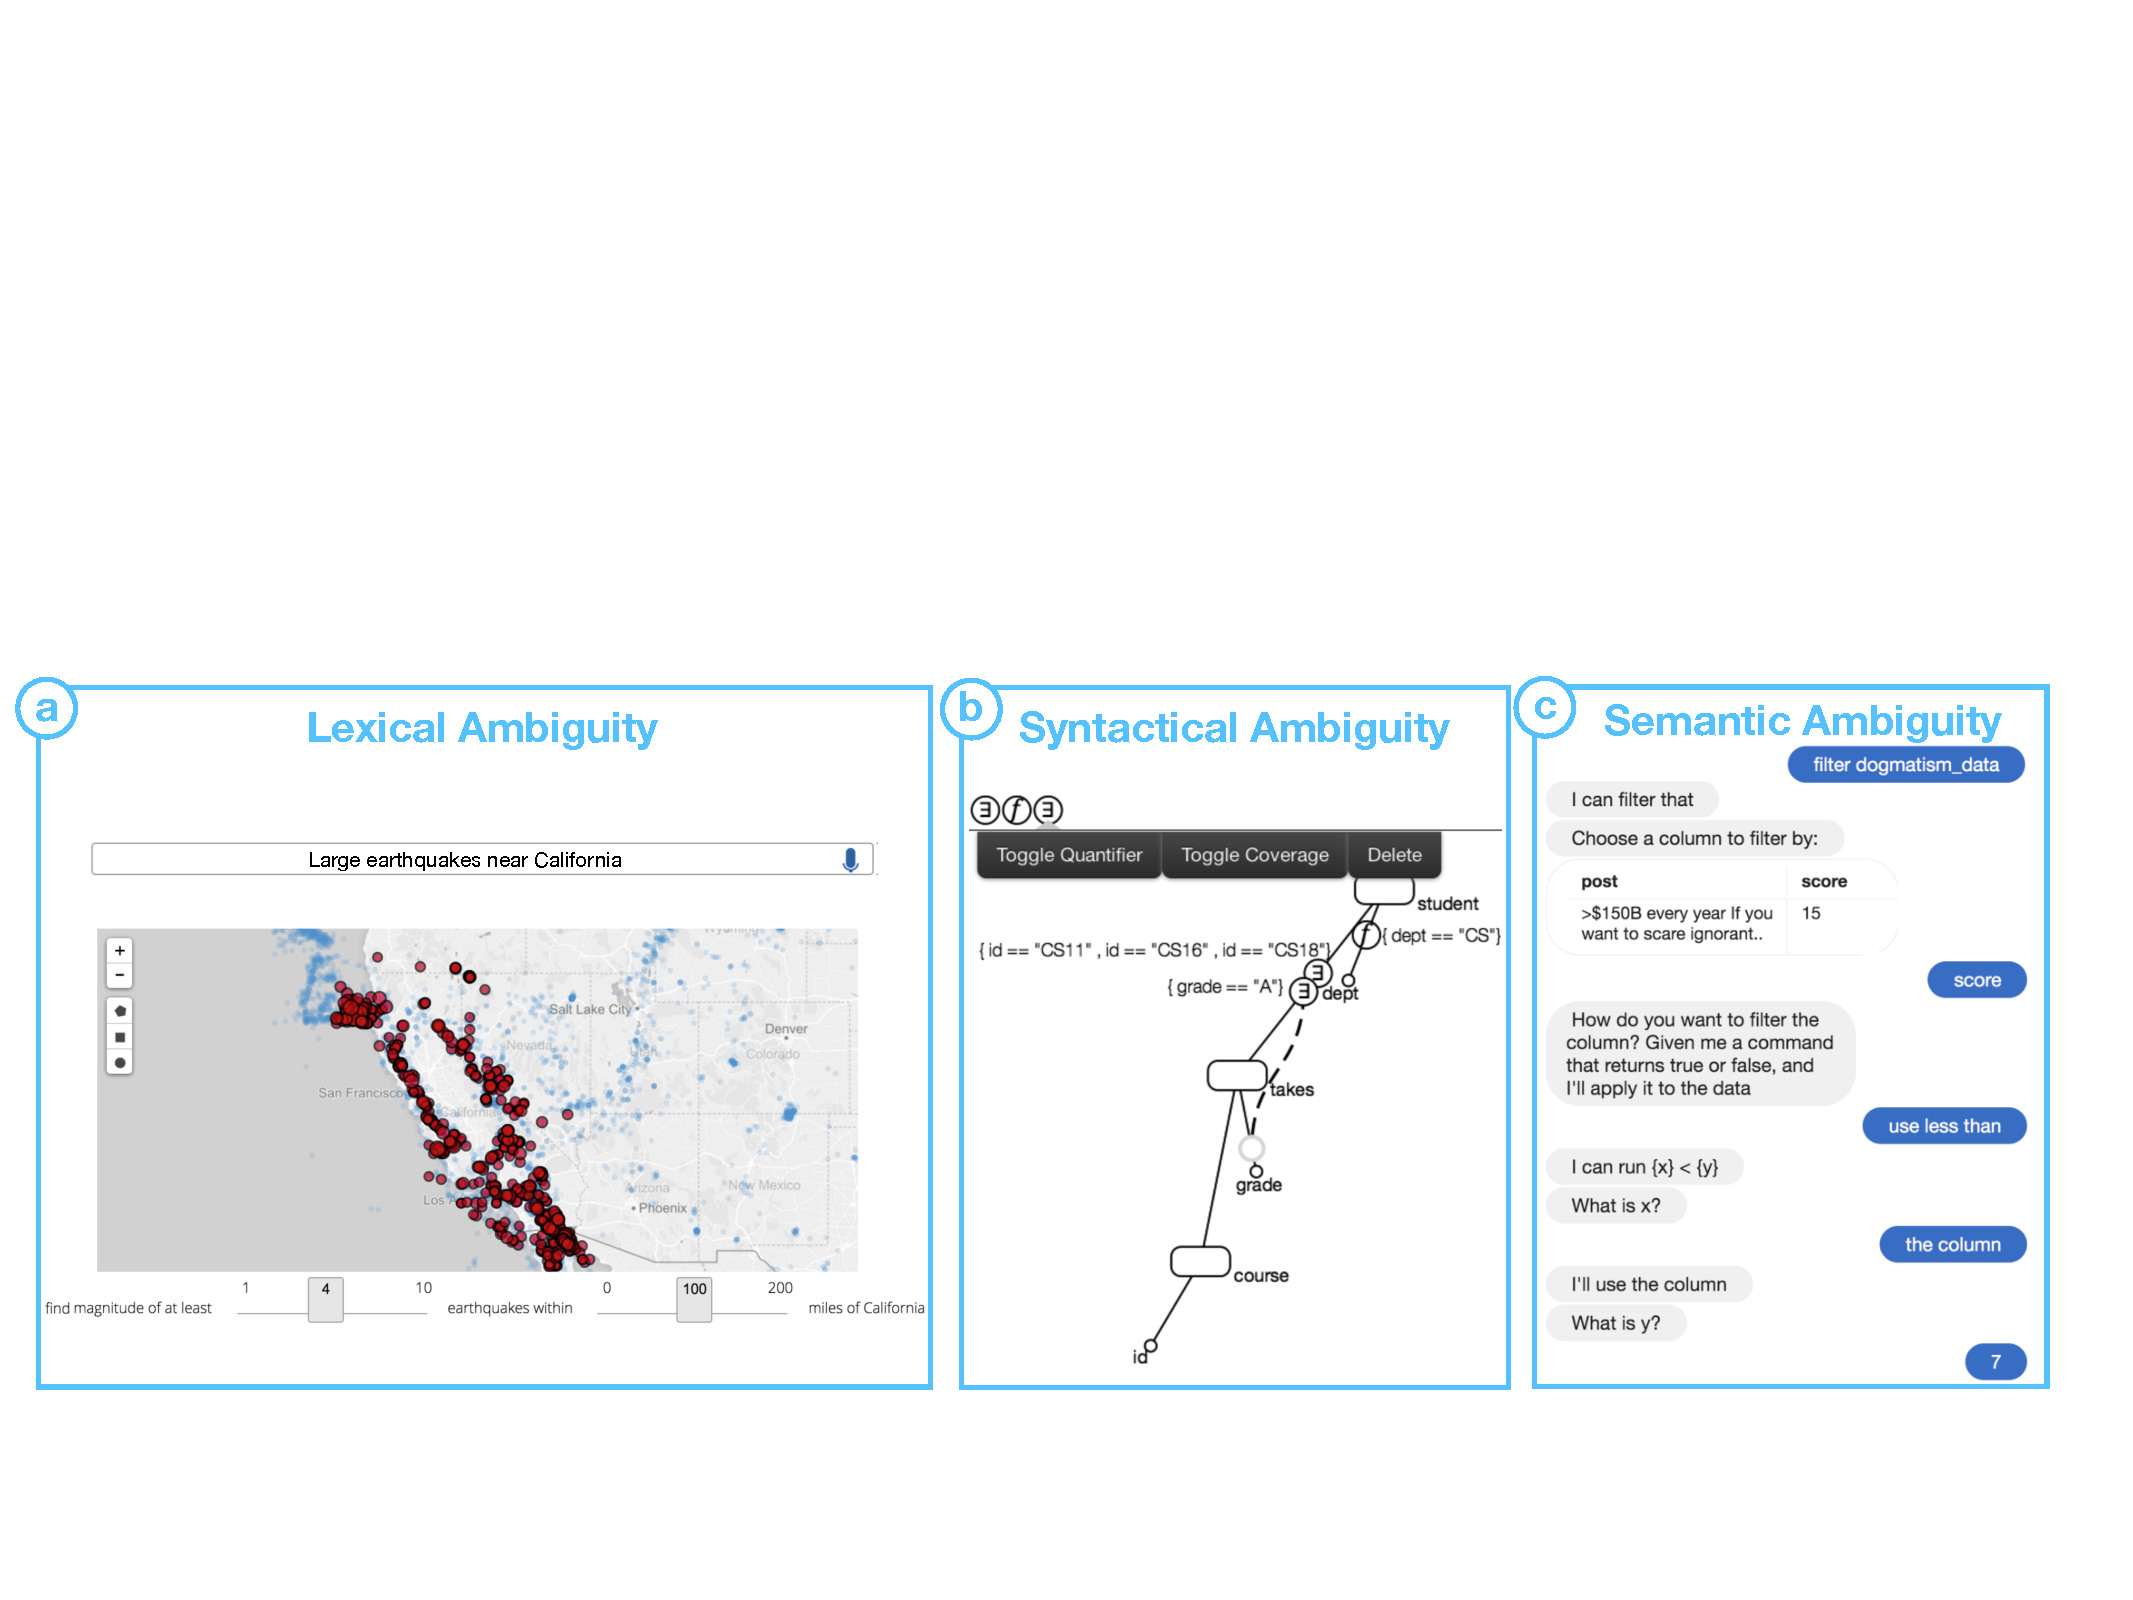
\includegraphics[width=\textwidth]{figures/ambiguity.pdf}
\caption{Examples of fuzzy, complex queries: a) Eviza~\cite{Setlur2016} uses ambiguity widgets to enable users to clarify vaguely-defined terms in their input query to resolve lexical ambiguity; b) DataPlay~\cite{Abouzied2012} allow users to toggle between `for all' and `at least one' quantifier to control for syntactical ambiguity; c) Iris~\cite{Fast2018} accepts a vague high-level task description and gather the additional information required through follow-up questions in a nested conversation.}
\label{fig:ambiguity}
\end{figure}
\stitle{Lexical Ambiguity}: Lexical ambiguity involves the use of vague descriptors in the input queries. Resolving these lexical ambiguities has been a subject of research in natural language interfaces for visualization specification, such as DataTone~\cite{Gao2015} and Eviza~\cite{Setlur2016}. These interfaces detect ambiguous quantifiers in the input query (e.g. ``Large earthquakes near California''), and then displays ambiguity widgets in the form of a widget to allow users to specify the definition of `large' in terms of magnitude and the number of miles radius for defining `near', as shown in Figure~\ref{fig:ambiguity}a. These ambiguity widgets not only serve as a way to provide feedback to the system for lexically vague queries, but is also a way for explaining how the system has interpreted the input queries. In addition to ambiguity in the filter descriptions, as we have seen in the \zv study, there is often also ambiguity in the terminologies used for describing query patterns. We have developed a tool, \ssearch~\cite{Siddiqui2018} that works on top of an internal shape query algebra to flexibly match visualization segments, such as a trendline that ``first rises and then go down''. After the translation to the internal query representation, \ssearch then performs efficient perceptually-aware matching of visualizations through grouping, pruning and sampling optimizations. Similarly the \vida framework, we envision  lexical ambiguity to be resolved by determining the appropriate \textit{parameters} to the internal \vidaql for achieving the user's desired querying effects.
\stitle{Syntactic Ambiguity}: Syntactic ambiguity is related to the vagueness in specifying how the query should be structured or ordered. For example, DataPlay introduced the idea of syntax non-locality in SQL, in which switching from an existential (at least one) to a universal (for all) quantifier requires major structural changes to the underlying SQL query~\cite{Abouzied2012}. As shown in Figure~\ref{fig:ambiguity}b, DataPlay consist of a visual interface that allowed users to directly manipulate the structure of the query tree in tweaking the query to its desired specification. In the \vida framework, syntactic ambiguities resolution involves mapping portions of the vague queries into to \textit{a series of multi-step workflows} to be executed in \vidaql and exposing feedback frameworks to allow users to directly tweak the internal query representation. %The query modification is done in a declarative manner in that the underlying mechanism in which the visualized workflow gets translated to the querying language is largely hidden from the end-user. 
\agp{I don't understand this. Can you give me an example of where syntactic ambiguity may arise, e.g., in ZQL?} 
\dor{In ZQL, something along the line of searching for something increasing in one collection and decreasing in another, the ambiguity is in whether to loop through two collections simultaneously and sort by a common objective, or find the top k in one collection first, then lowest-k in another collection to find the desired visualization. Essentially syntactic ambiguity happens when there is ambiguity in how the sequence of operations should be carried out is vague or unspecified.}

\stitle{Semantic Ambiguity}: Semantic ambiguity includes addressing `why' questions that are logically difficult to answer, such as `why do these datapoints look different from others?'. For example, Scorpion~\cite{Wu2013} traces the provenance of a set of input data tuples to find predicates that explain the outlier behavior. Semantic ambiguity can also arises when the user does not specify their intent completely or explicitly, which is often the case in early stages of visual data exploration. Natural language interface for visual data exploration, such as Evizeon~\cite{Hoque2017} makes use of anaphoric references to fill in incomplete follow-on queries. For example, when a user says `Show me average price by neighborhood', then `by home type', the system interprets the anaphoric reference as continuing the context of the original utterance related to average price on the y-axis. Semantic ambiguity can often be composed of one or more lexical and syntactical ambiguity. For example, in Iris~\cite{Fast2018}, a user can specify a vague, high-level query such as `Create a classifier', then Iris makes use of nested conversations to inquire about what type of classifier to chose and what features to use in the model to fill in the details of the structure and parameters required. 

\agp{cite causality work~\cite{meliou2010causality,roy2014formal}}
%If a semantically vague query is not expressible through existing \vidaql, more research may be necessary for developing novel discovery modules in the \vida ecosystem. %, since the operations involved in the query may not be covered by the limited workflow combinations in the PVQS. 

% Another form of syntactic ambiguity is how  through followup query tweaking 
% nested queries and anaphoric references~\cite{Hoque2017}. Show me relationship between price and -----, then "Break down by -----".
% user intention, composition , Accounting for user interaction, mental models. More global objective taking into account user with the goal of dataset understanding rather than task completion. Need for a unified framework of inference to take all of these into account (e.g. natural language, etc)